\section{Performance dimension: Core architecture}

For the core-level analysis, we ask to which degree the code exploits the particular microarchitecture of the chip efficiently:
Does it make use of the (most) advanced instruction set, and does it exploit the memory interconnect properly?
The instruction set usage is something we can evaluate per core.
Caches on chips however are designed to serve all hardware threads on their chips.
We will not be able to assess if we use them efficiently if we use only one core.
We have to run the benchmark over the whole node.
Therefore, this section is not called ``core'', but we call it ``core architecture''.



\begin{figure}
 \begin{center}
  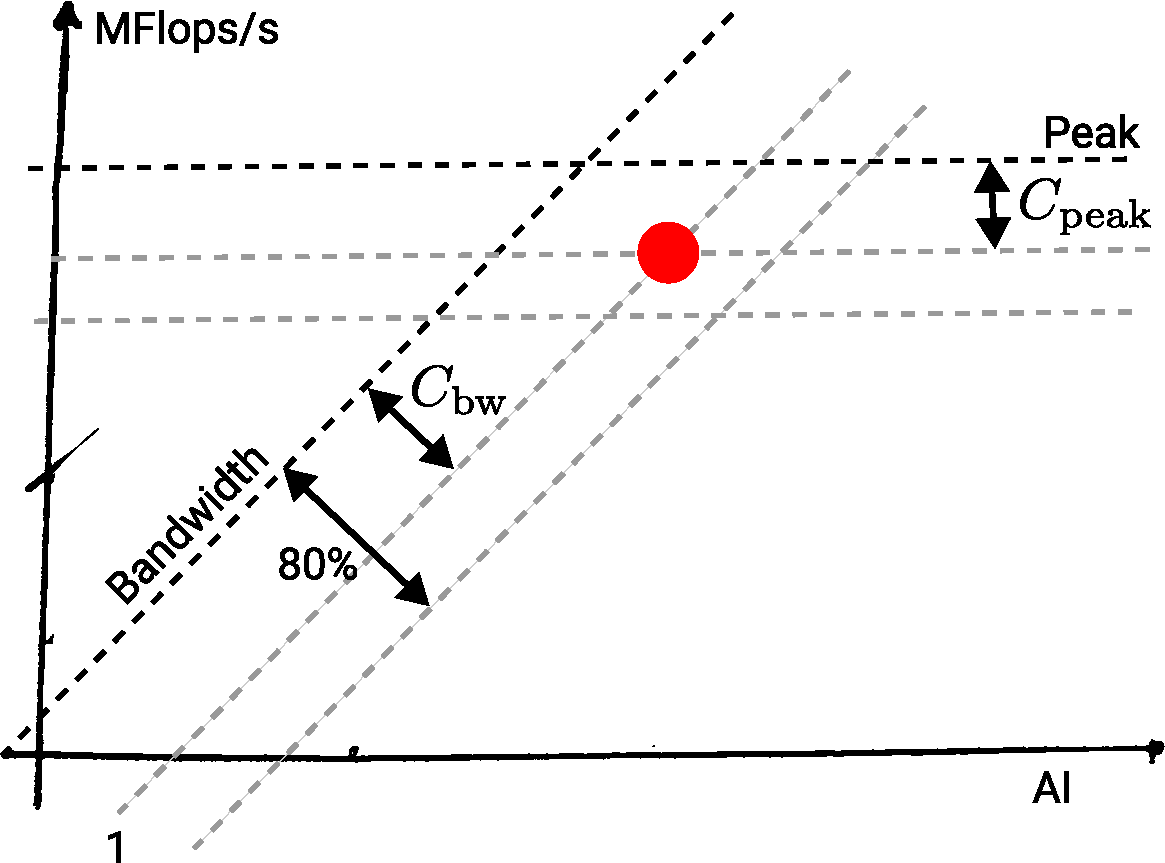
\includegraphics[width=0.7\textwidth]{high-level/core-architecture.pdf}
 \end{center}
 \caption{
  Schematic illustration of a roofline analysis of a code.
  We illustrate the peak performance threshold (dark dotted horizontal line) and the maximum bandwidth (diagonal).
  The code's actual compute performance delivered and memory bandwidth used is by a factor of $C_{\text{peak}}$ or $C_{\text{bw}}$ respectively lower than these maximum thresholds.
  \label{figure:core-architecture}
 }
\end{figure}


Our method of choice to argue about the core architecture usage is a very simple variant of the roofline model (Figure~\ref{figure:core-architecture}).
We know the maximum memory bandwidth of the system over the arithmetic intensity (AI).
This gives us the roofline's diagonal line that serves as a natural threshold: 
We cannot get more data through the system besides temporary outliers if we make really good use of caches.
The peak performance of the chip serves as a further, this time hard upper bound for our performance.
It yields the horizontal line. 


Once we know the throughput and performance delivered by our code, we can draw parallel lines to these two thresholds that match our observations:
As long as they are ``only'' by a factor of $C_{\text{bw}} \geq 80\%$ or $C_{\text{bw}} \geq 60\%$ lower than the maximum lines, i.e.~as long as we we stay within a 60\% or 80\% corridor, all is fine.



\paragraph{Benchmark preparation}

Throughout this assessment, we use one fixed problem setup.
It has to be reasonably demanding such that it makes sense to exploit all threads of the node plus it computes something reasonable.

\begin{assessmentcrime}
 We assess a setup that fits completely into one of the caches.
\end{assessmentcrime}


\begin{assessmentcrime}
 We study a code that is not translated with the most aggressive compiler optimisation for the particular architecture that we study. 
\end{assessmentcrime}


\paragraph{Data collection}

Nobody will be able to exploit all caches with only one core!



 
\paragraph{Evaluation}

We use the two quantities $C_{\text{bw}}$ and $f_{\text{peak}}$ to determine if we consider the code to have a core architecture flaw:

\begin{center}
 \begin{tabular}{r|p{0.22\textwidth}p{0.22\textwidth}p{0.22\textwidth}}
  & $C_{\text{bw}}\geq 0.8$ & $0.8 > C_{\text{bw}}\geq 0.6$ & $0.6 > C_{\text{bw}}$ \\
  \hline
  $f_{\text{peak}} \geq 0.8$
   & \cellcolor{green!25}
   & \cellcolor{orange!25}
   & \cellcolor{red!25}
  \\
  $0.8 > f_{\text{peak}} \geq 0.6$
   & \cellcolor{orange!25}
   & \cellcolor{orange!25} flaw
   & \cellcolor{red!25}
  \\
  $0.6 > f_{\text{peak}}$
   & \cellcolor{red!25}
   & \cellcolor{red!25}
   & \cellcolor{red!25} severe flaw
 \end{tabular}
\end{center}

%{equation:intra-node:performance-model}

\begin{performancemetric}
 If $C_{\text{bw}}< 0.8$, the implementation does not use the memory subsystem sufficiently, i.e.~we fail to bring enough data into the chip.
 If $C_{\text{bw}}< 0.6$, this problem is severe.
\end{performancemetric}


\begin{performancemetric}
 If $f_{\text{peak}}< 0.8$, the code does not use the compute units properly.
 If $f_{\text{peak}}< 0.6$, the problem is significant.
\end{performancemetric}


\paragraph*{How it works}

\begin{itemize}[noitemsep]
  \item[$\boxplus$] Run a standard benchmark to determine a realistic maximum throughput (bandwidth) and peak performance.
  \item[$\boxplus$] Assess your code to find out if it makes sufficient use of the available bandwidth and compute units.
\end{itemize}


\paragraph*{How it does not work}

\begin{itemize}[noitemsep]
  \item[$\boxminus$] Apply some performance counters as a black box without a roofline model.
  \item[$\boxminus$] Run the roofline model for individual functions or loops and make statements on the overall code.
\end{itemize}


